\paragraph{QuizziPedia::Front-End::Directives::QuestionTextDirective}

\label{QuizziPedia::Front-End::Directives::QuestionTextDirective}

\begin{figure}[ht]
	\centering
	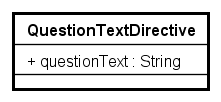
\includegraphics[scale=0.80,keepaspectratio]{UML/Classi/Front-End/QuizziPedia_Front-end_Directives_QuestionTextDirective.png}
	\caption{QuizziPedia::Front-End::Directives::QuestionTextDirective}
\end{figure} 
\FloatBarrier

\begin{itemize}
	\item \textbf{Descrizione}: rappresenta il componente grafico che permette all'utente di scrivere o modificare il testo di una domanda;
	\item \textbf{Utilizzo}: viene usato per permettere all'utente di scrivere o modificare il testo di una domanda;
	\item \textbf{Relazioni con altre classi}: 
	\begin{itemize}
		\item \textbf{OUT \texttt{TrueFalseQuestionsView}}: \textit{view\ped{G}} contenente i campi per creare una domanda vero/falso; 
		\item \textbf{OUT \texttt{MultipleQuestionsView}}: \textit{view\ped{G}} contenente i campi per creare una domanda a risposta multipla;
		\item \textbf{OUT \texttt{ConnectionQuestionsView}}: \textit{view\ped{G}} contenente i campi per creare una domanda a collegamento;
		\item \textbf{OUT \texttt{ImagesSortingQuestionsView}}: \textit{view\ped{G}} contenente i campi per creare una domanda a ordinamento immagini;
		\item \textbf{OUT \texttt{StringsSortingQuestionsView}}: \textit{view\ped{G}} contenente i campi per creare una domanda a ordinamento stringhe;
		\item \textbf{OUT \texttt{FillingQuestionsView}}: \textit{view\ped{G}} contenente i campi per creare una domanda a riempimento testo;
		\item \textbf{OUT \texttt{ClickableAreaQuestionsView}}: \textit{view\ped{G}} contenente i campi per creare una domanda ad area cliccabile.
	\end{itemize}
	\item \textbf{Attributi}: 
	\begin{itemize}
		\item \texttt{+ questionText: String} \\ Attributo contenente il testo della domanda.
	\end{itemize}
\end{itemize}